\documentclass[12pt,a4paper]{article}
\usepackage[polish]{babel}
\usepackage[T1]{fontenc}
\usepackage[utf8x]{inputenc}
\usepackage{hyperref}
\usepackage{url}
\usepackage[]{algorithm2e}
\usepackage{listings}
\usepackage{graphicx}
\usepackage{color}
\usepackage{listings}
\usepackage{fancyhdr}
\usepackage{pgfplots}
\usepackage{pgf-pie} 
\usepackage{newtxtext,newtxmath}
\usepackage{float}
\usepackage{amsmath}
\usepackage{caption}
\usepackage{multirow}
\usepackage{colortbl}
\usepackage{hhline}

\pgfplotsset{compat=1.18}

\lstloadlanguages{% Check Dokumentation for further languages ...
	C,
	C++,
	csh,
	Java
}

\definecolor{red}{rgb}{0.6,0,0} % for strings
\definecolor{blue}{rgb}{0,0,0.6}
\definecolor{green}{rgb}{0,0.8,0}
\definecolor{cyan}{rgb}{0.0,0.6,0.6}

\newtheorem{twr}{Twierdzenie}

\lstset{
	language=csh,
	basicstyle=\footnotesize\ttfamily,
	numbers=left,
	numberstyle=\tiny,
	numbersep=5pt,
	tabsize=2,
	extendedchars=true,
	breaklines=true,
	frame=b,
	stringstyle=\color{blue}\ttfamily,
	showspaces=false,
	showtabs=false,
	xleftmargin=17pt,
	framexleftmargin=17pt,
	framexrightmargin=5pt,
	framexbottommargin=4pt,
	commentstyle=\color{green},
	morecomment=[l]{//}, %use comment-line-style!
	morecomment=[s]{/*}{*/}, %for multiline comments
	showstringspaces=false,
	morekeywords={ abstract, event, new, struct,
		as, explicit, null, switch,
		base, extern, object, this,
		bool, false, operator, throw,
		break, finally, out, true,
		byte, fixed, override, try,
		case, float, params, typeof,
		catch, for, private, uint,
		char, foreach, protected, ulong,
		checked, goto, public, unchecked,
		class, if, readonly, unsafe,
		const, implicit, ref, ushort,
		continue, in, return, using,
		decimal, int, sbyte, virtual,
		default, interface, sealed, volatile,
		delegate, internal, short, void,
		do, is, sizeof, while,
		double, lock, stackalloc,
		else, long, static,
		enum, namespace, string},
	keywordstyle=\color{cyan},
	identifierstyle=\color{red},
}

\usepackage{caption}
\DeclareCaptionFont{white}{\color{white}}
\DeclareCaptionFormat{listing}{\colorbox{blue}{\parbox{\textwidth}{\hspace{15pt}#1#2#3}}}
\captionsetup[lstlisting]{format=listing,labelfont=white,textfont=white, singlelinecheck=false, margin=0pt, font={bf,footnotesize}}


\addtolength{\hoffset}{-1.5cm}
\addtolength{\marginparwidth}{-1.5cm}
\addtolength{\textwidth}{3cm}
\addtolength{\voffset}{-1cm}
\addtolength{\textheight}{2.5cm}
\setlength{\topmargin}{0cm}
\setlength{\headheight}{0cm}

\newcommand\blankpage{%
    \null
    \thispagestyle{empty}%
    \addtocounter{page}{-1}%
    \newpage}

\begin{document}

    \pagestyle{fancy}
    \rhead{\textit{Projekt systemu przechowywania danych dla sklepu}}

    \title{
    \vspace*{3cm}
    \textbf{Projekt systemu przechowywania danych dla sklepu}}
    \author{Adam Paździerz\\ Dawid Wydra\\ Jakub Gurgul\\ Mariusz Pyrk\\ 
            \vspace*{0.5cm} \\      
            Programowanie Obiektowe i Graficzne\\
            \textit{Informatyka - profil praktyczny}\\
            Wydział Matematyki Stosowanej\\
            \textbf{Politechnika Śląska}\\
            Gliwice, Polska
    }
    \date{\today}
	
	\maketitle
	\newpage

    \tableofcontents
    \thispagestyle{empty}
    \newpage
\section{Wstęp}

    \subsection{Cel}
        Celem projektu jest stworzenie aplikacji umożliwiającej zarządzanie siecią aptek. Aplikacja posiada połączenie z rozbudowaną bazą danych, która zawiera wszystkie niezbędne informacje i dane potrzebne do funkcjonowania sieci sklepów. Program przeznaczony jest dla pracowników sklepu. Pomoże nadzorować pracę firmy w wielu jej aspektach: dostawy, dystrybucja produktów, zarządzanie umowami, logowanie
            pracowników oraz klientów.
            
    \subsection{Założenia}
        Przed przystąpieniem do wykonania, przemyślano jakie cele powinna spełniać aplikacja oraz baza danych dla sieci sklepów, tak aby móc jak najefektywniej spełniać swoje zadanie. Podstawowe założenia to możliwość logowania użytkowników oraz pozyskiwanie informacji o poniższych aspektach firmy:
        \begin{enumerate}
            \item \textbf{Pracownicy} - obsługa pensji, podpisanych umów, przydzielonego stanowiska, danych personalnych oraz poświadczeń bezpieczeństwa;
            \item \textbf{Sklepy} - identyfikacja pracowników przypisanych do placówki, sprawdzenie stanu magazynowego oraz obsługiwanych zamówień;
            \item \textbf{Klienci} - dane kontaktowe oraz adres do dostawy, złożone zamówienia;
            \item \textbf{Zamówienia} - sumaryczna kwota, zamówione produkty, pracownik oraz sklep obsługujący;
            \item \textbf{Produkty} - ilość sztuk na stanie, przypisane dostawy oraz cena jednostkowa;
            \item \textbf{Dostawcy} - spis oraz artykuły które dostarczają;
            \item Aplikacja będzie pozwalała na zalogowanie się pracownika do systemu, i zgodnie ze swoim stanowiskiem na przejrzenie aktywnych zleceń, sprawdzenie stanu magazynowego sklepu, swoich umów, umów sklepu lub całej sieci, sprawdzić oraz dodać nowych pracowników, klientów i dostawców;
            \item Przewidujemy trzy poziomy dostępu dla pracowników: sprzedawca, kierownik sklepu oraz kierownik regionalny.
        \end{enumerate}
            
    
\section{Wdrożenie}
    \subsection{Aplikacja}
        Aplikacja została wykonana w języku C\#, z wykorzystaniem \textit{Windows Presentation Foundation} (WPF) w celu generowania widoku aplikacji. Program został napisany w oparciu o model \textit{Model–view–viewmodel} (MVVM). Stworzony panel przedstawia widok na bazę danych z poziomu administratora informatycznego. Widzi on wszystkie tabele i zależności oraz ma nieograniczone możliwości ingerencji w tabelę.
            
    \subsection{Baza danych}
        Została wykonana z zachowaniem wsyztskich założeń, które zostały dla niej stworzone w tej dokumentacji. Została wypełniona losowymi danymi z wykorzystaniem strony \href{https://www.mockaroo.com/}{mockaroo.com}, która umożliwa generowanie losowych danych w określonych typach, (np. Imię, Nazwisko czy Miasto). Poniżej zamieszamy zrzut ekranu z aplikacji phpMyAdmin prezentujący ostateczny wygląd bazy oraz relacje w niej panujące. W celu zwiększenia użyteczności bazy, stworzono dwa widoki odpowiedzialne za połączenie zamówień z klientami, sklepami, produktami i pracownikami. Drugi widok odpowiada za połączenie produktów z dostawcami, przedstawienie cen zakupu oraz nazw produktów i dostawców, widok ten wyświetlany jest w zakładce produktów oraz dostawców. 
            
        \begin{figure}[H]
            \centering
            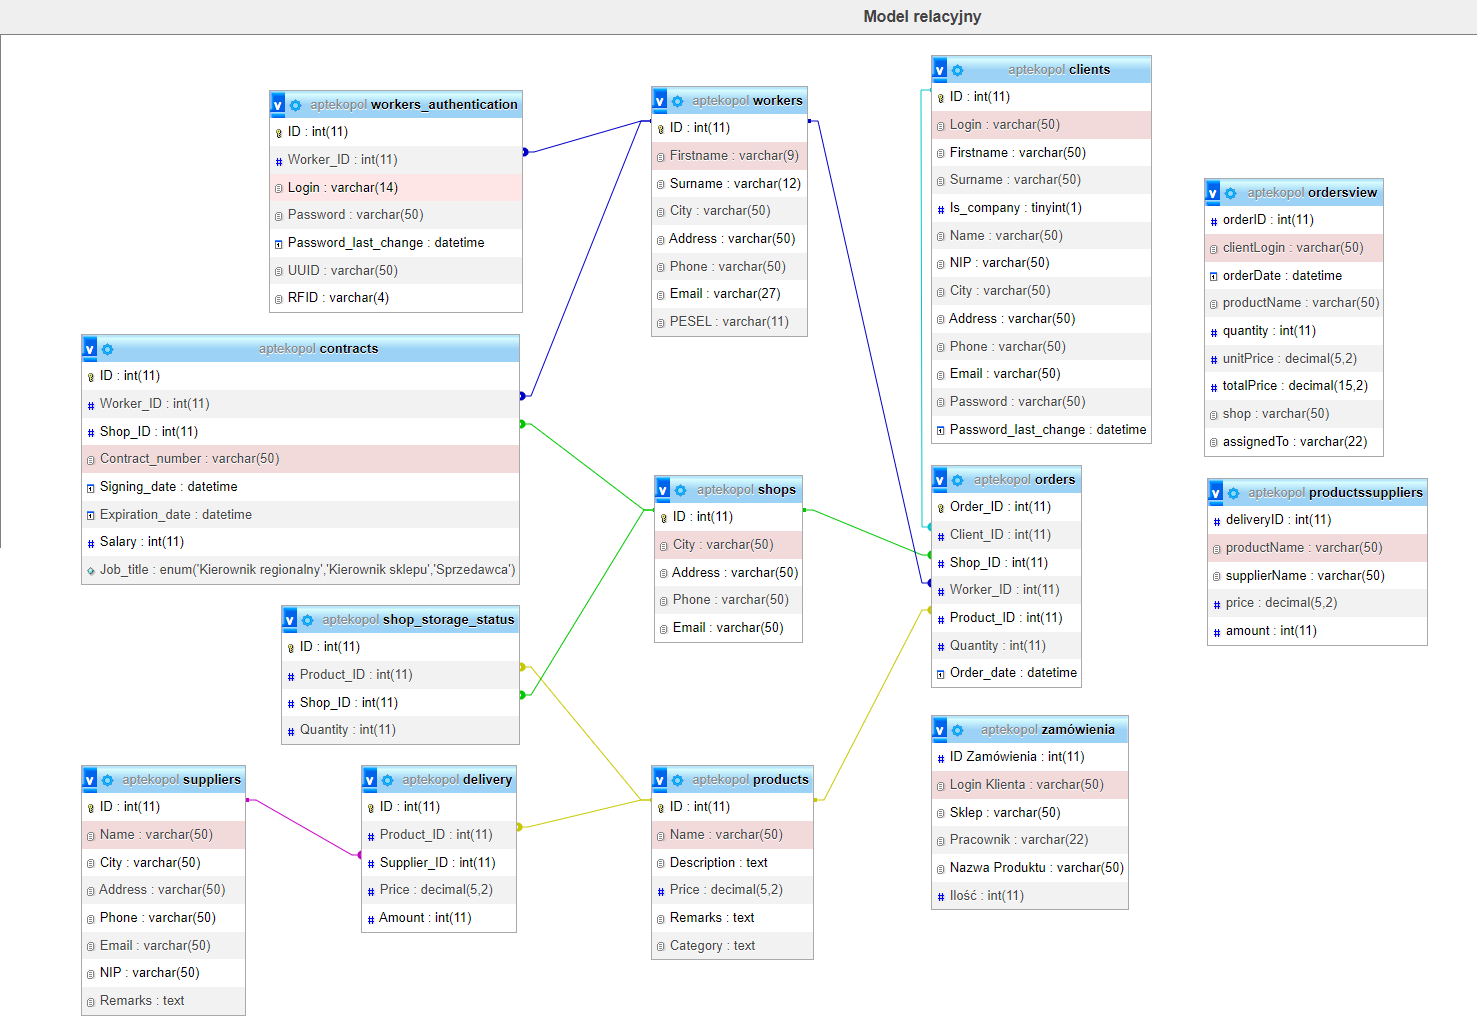
\includegraphics[scale=0.4]{images/phpmyadmin.png}
            \caption{Zrzut ekranu z aplikacji phpMyAdmin, prezentujący model relacyjny}
        \end{figure}
                 
    \subsection{Połączenie z bazą}
        \begin{enumerate}
            \item Z poziomu phpmyadmin tworzymy bazę danych, koniecznie z takim kodowaniem
                
                \begin{figure}[H]
                    \centering
                    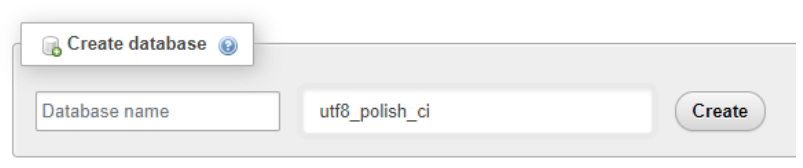
\includegraphics[scale=0.4]{images/kodowanie.png}
                    \caption{Zrzut ekranu kodowania bazy danych}
                \end{figure}
                    
            \item Będąc w naszej bazie danych, z zakładki import wybieramy plik aptekopol.sql
                
                \begin{figure}[H]
                    \centering
                    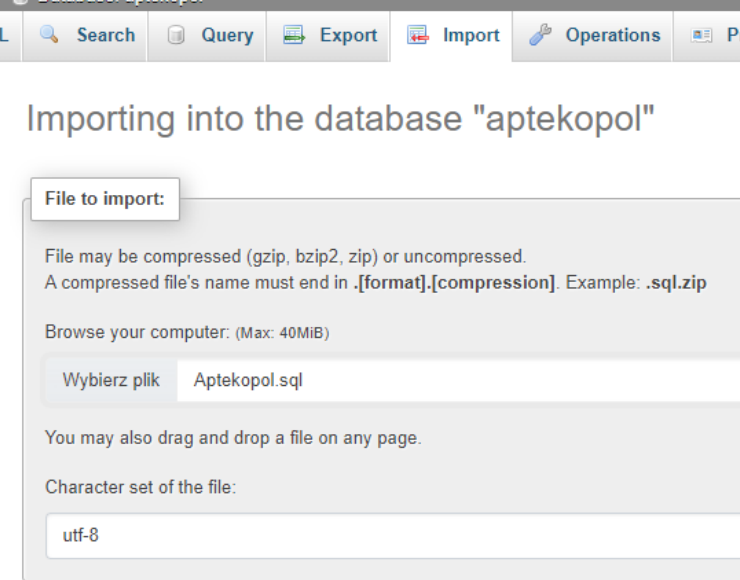
\includegraphics[scale=0.4]{images/import.png}
                    \caption{Zrzut ekranu importowania bazy danych}
                \end{figure}
                    
            \item Z poziomu projektu w VS Studio, wybieramy settings, pola powinny być już uzupełnione jeśli nie to wypełniamy je w ten sam sposób, jedynie pole z nazwą użytkownika i hasłem może być inne, domyślnie jest root bez hasła.
                
                \begin{figure}[H]
                    \centering
                    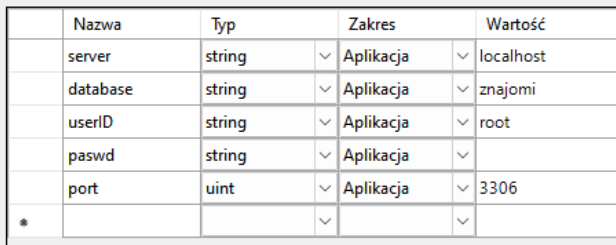
\includegraphics[scale=0.4]{images/settings.png}
                    \caption{Zrzut ekranu ustawień z programu Visual Studio}
                \end{figure}
                
            \item XAMMP cały czas musi działać w tle, port (domyślnie) 3306
                
                \begin{figure}[H]
                    \centering
                    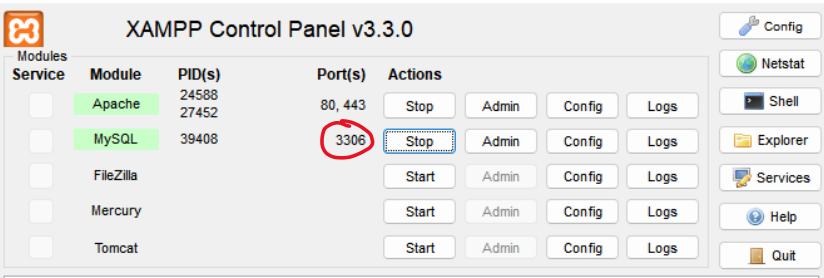
\includegraphics[scale=0.4]{images/xampp.png}
                    \caption{Zrzut ekranu ustawień aplikacji xampp}
                \end{figure}
                    
            \item Po skompilowaniu projektu w VS Studio powinno nastąpić połączenie z bazą danych
                    
        \end{enumerate}
        
    \subsection{Model obiektowy i diagram UML}
        \begin{figure}[H]
            \centering
            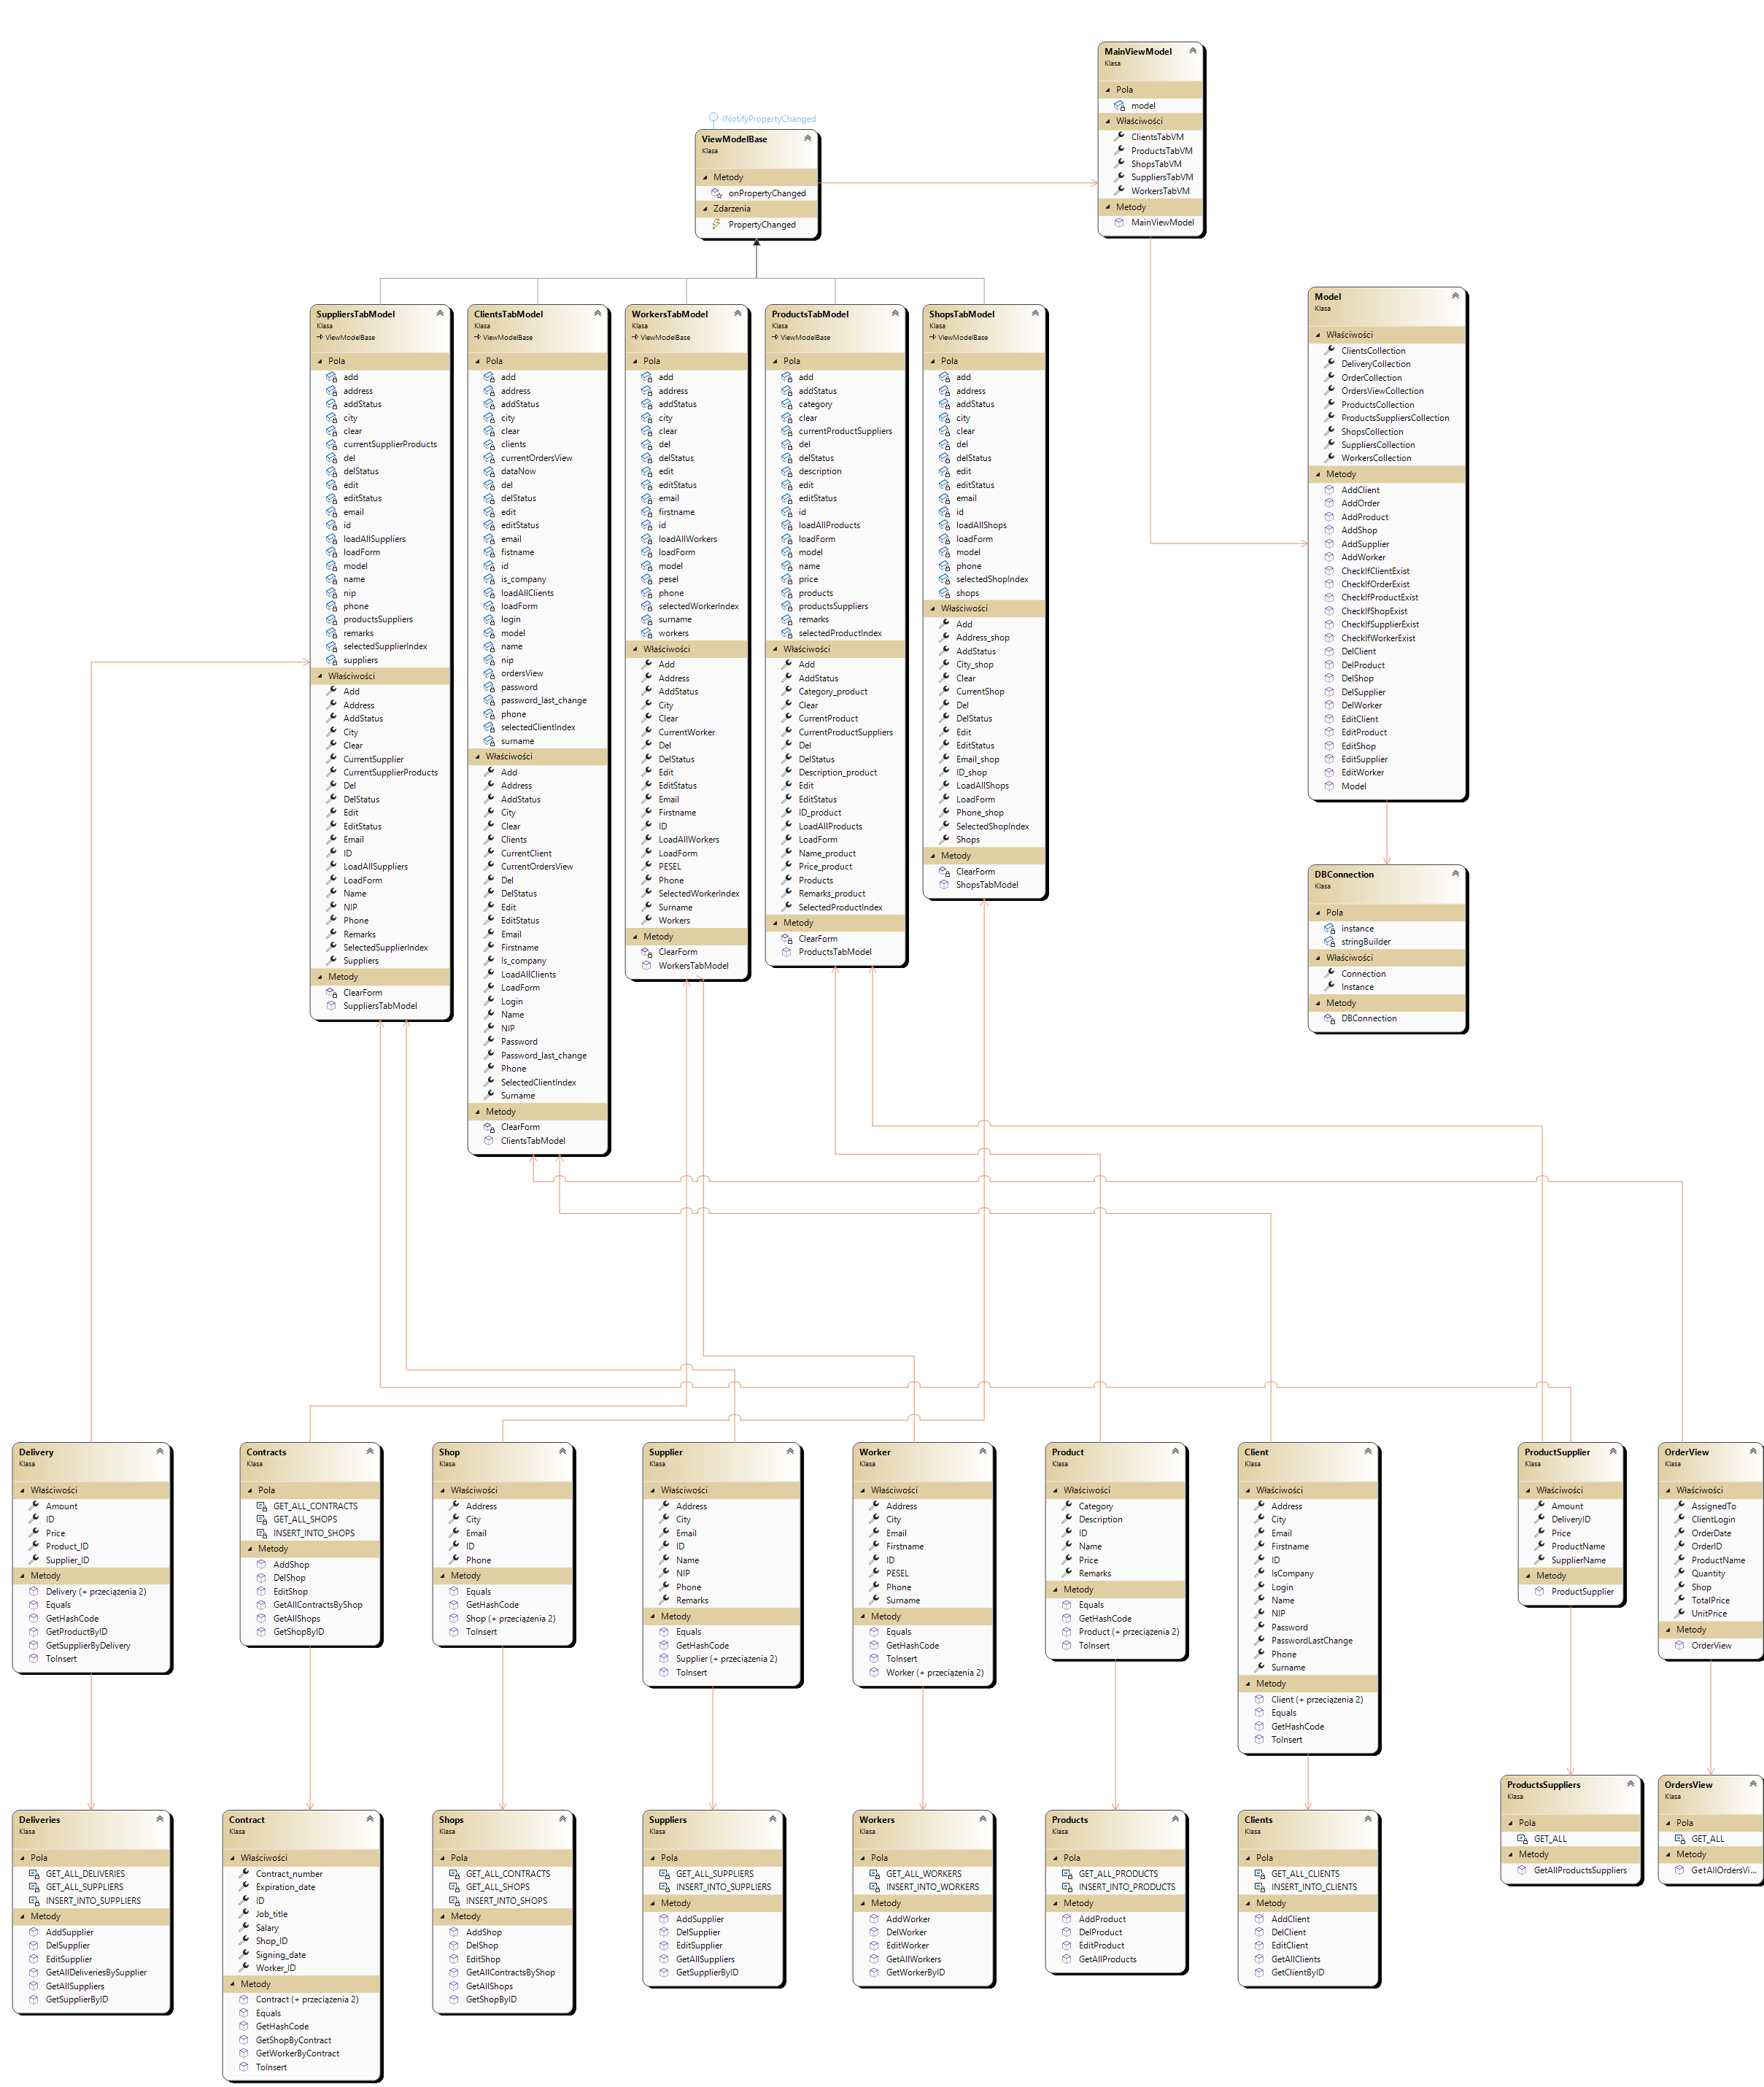
\includegraphics[width=\textwidth]{images/ClassDiagram1.png}
            \caption{Diagram UML aplikacji}
        \end{figure}
        
    \subsection{Wygląd aplikacji i funkcjonalności}
        Stworzona przez nas aplikacja pozwala na zarządzanie pracownikami (edycje, dodawanie oraz usuwanie), zarządzanie sklepami w sieci, zarządzanie produktami oraz podgląd łańcuchów dostaw dla konkretnych produktów, zarządzanie klientami (edycja oraz możliwość podglądu złożonych zamówień) oraz zarządzanie dostawcami (podgląd oraz edycja).
            
        \begin{figure}[H]
            \centering
            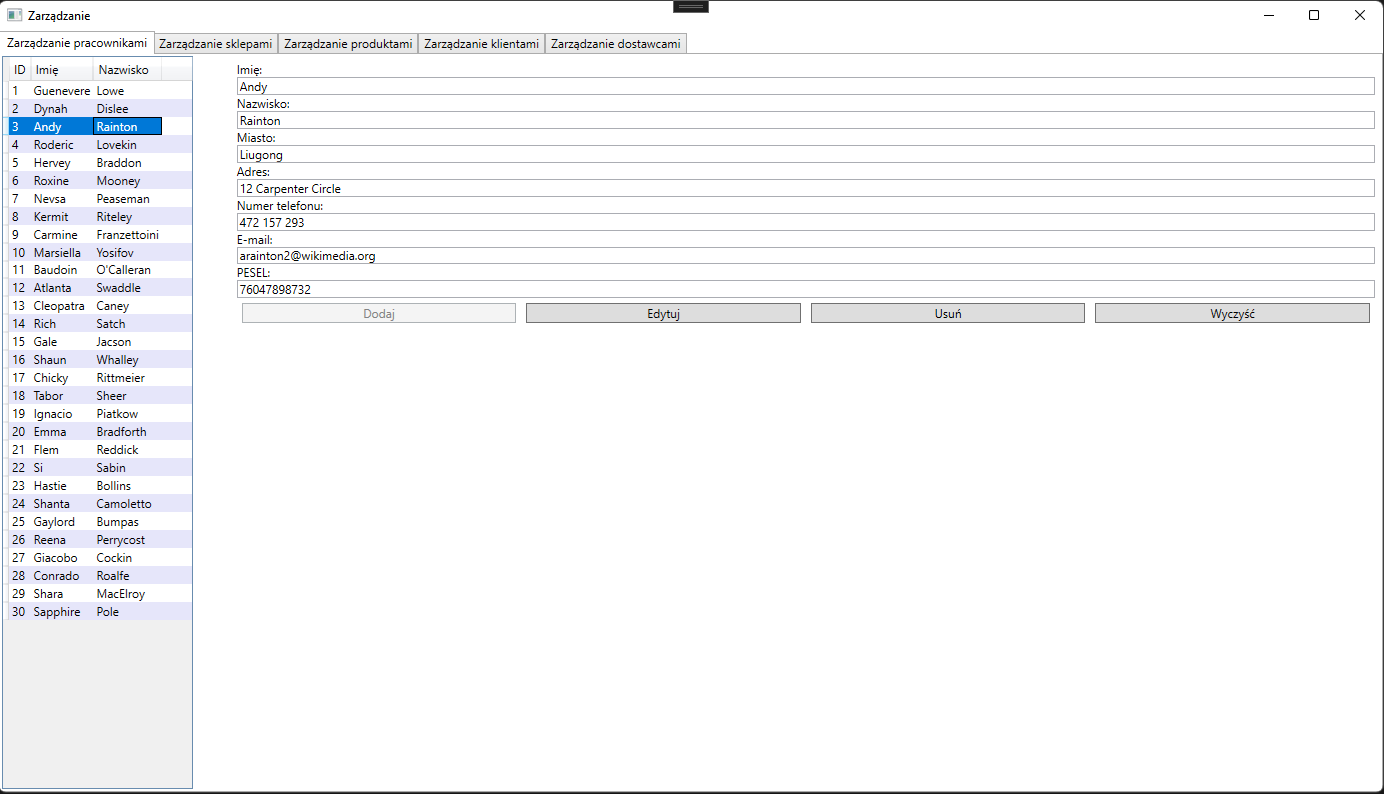
\includegraphics[scale=0.4]{images/pracownicy.png}
            \caption{Zrzut ekranu z aplikacji przedstawiający widok zakładki pracownicy}
        \end{figure}
            
        \begin{figure}[H]
            \centering
            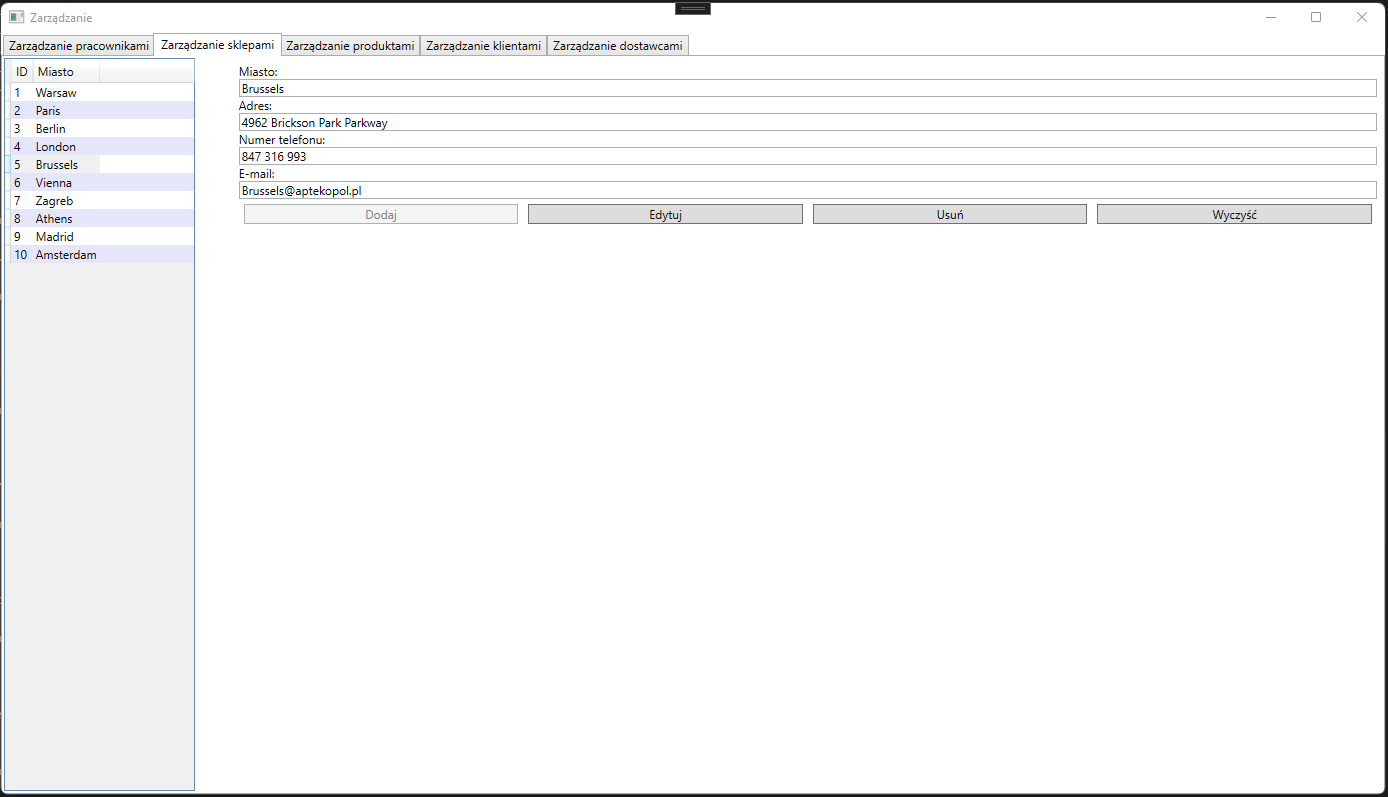
\includegraphics[scale=0.4]{images/sklepy.png}
            \caption{Zrzut ekranu z aplikacji przedstawiający widok zakładki sklepy}
        \end{figure}
            
        \begin{figure}[H]
            \centering
            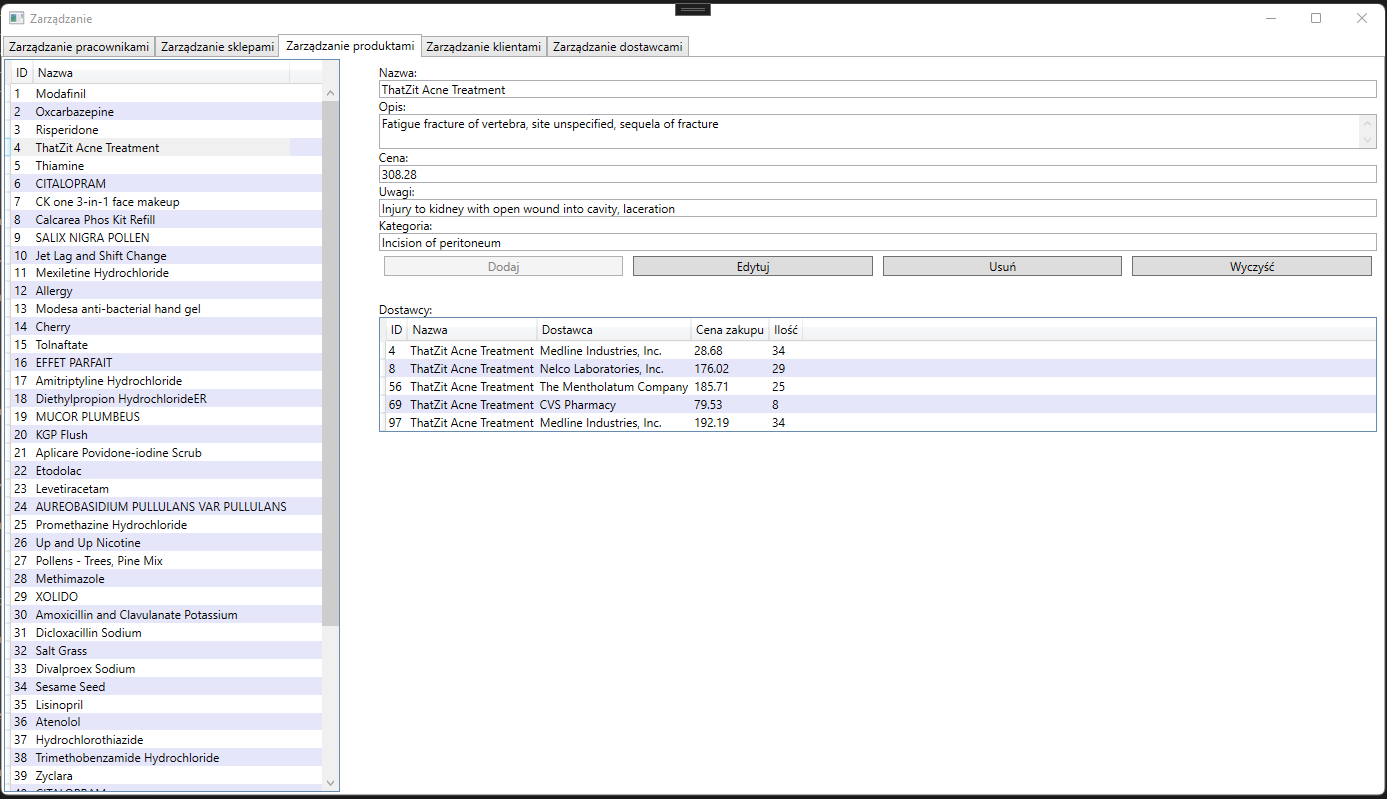
\includegraphics[scale=0.4]{images/produkty.png}
            \caption{Zrzut ekranu z aplikacji przedstawiający widok zakładki produkty}
        \end{figure}
            
        \begin{figure}[H]
            \centering
            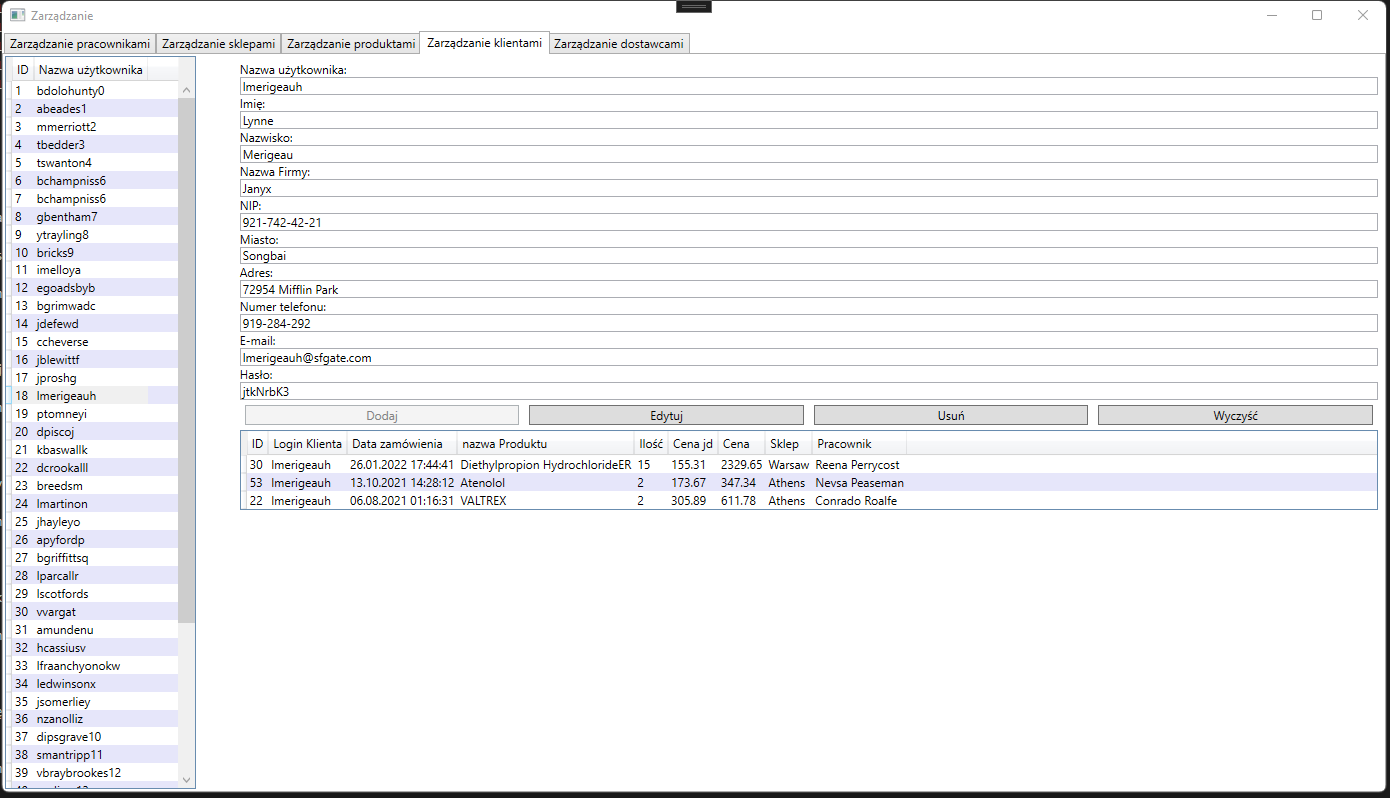
\includegraphics[scale=0.4]{images/kienci.png}
            \caption{Zrzut ekranu z aplikacji przedstawiający widok zakładki klienci}
        \end{figure}
            
        \begin{figure}[H]
            \centering
            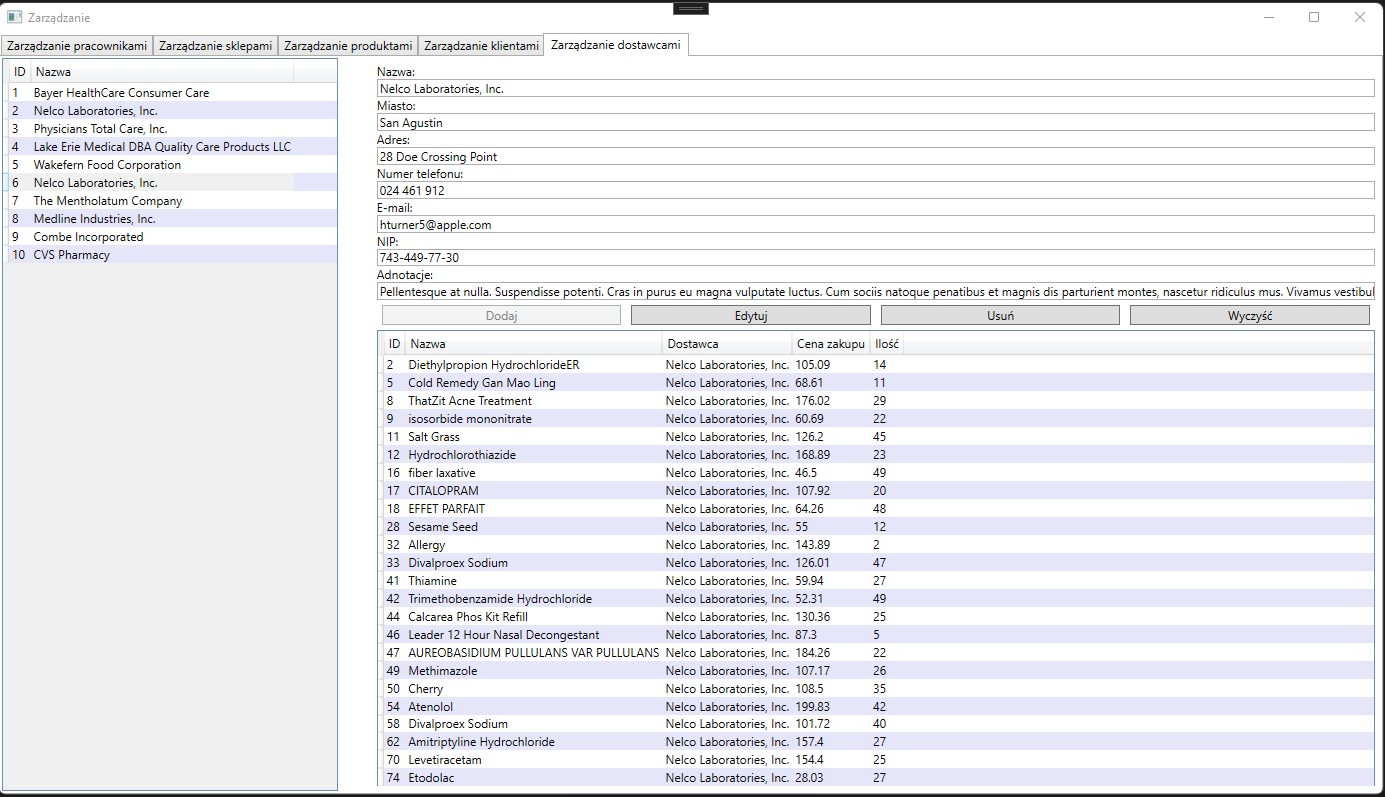
\includegraphics[scale=0.4]{images/dostawy.png}
            \caption{Zrzut ekranu z aplikacji przedstawiający widok zakładki dostawcy}
        \end{figure}
            
        \begin{figure}[H]
            \centering
            
\includegraphics{images/komunikat1.png}
            \caption{Komunikat wyświetlany po poprawnej edycji rekordu}
        \end{figure}
            
        \begin{figure}[H]
            \centering
            
\includegraphics{images/komunikat2.png}
            \caption{Komunikat przy próbie usunięcia rekordu który ma powiązania z innymi, na przykładzie usunięcia sklepu z przypisanymi pracownikami i zamówieniami}
        \end{figure}
        
\section{Podsumowanie i wnioski}
    \subsection{Podsumowanie projektu}
        Dzieki projektowi nauczyliśmy się lepieiej projektować tego typu aplikację. Najważniejszym doświadczeniem wyniesionym zprojektu było jego odpowiednie zaplanowanie przed przystąpieniem do prac. Dzięki dobrze wykonanym diagrmamo praca była prostrza i bardziej usestymatyzowana. Również dzięki wzorcowi MVVM było nam prościej rozdzielać poszczególne warstwy projektu. Pomogło to w szybszych zamianach i odnajdywaniu problemów pomiędzy warstwami. Po zakończeniu projektu o wiele lepiej znajdywaliśmy się w strukturze aplikacji, oraz w całym wzorcu MVVM. Dodatkowym aspektem który mogliśmy przećwiczyć, było połączenie z bazą danych oraz jej zarządzanie z poziomu aplikacji klienckiej i możliwość wykorzystania wiedzy nabytej na przedmiocie Bazy Danych.
            
    \subsection{Rozwój}
        Dodanie linków do zdjęć produktów, w celu ich szybszej identyfikacji przez klienta i pracownika. Możliwość sprawdzania obrotów sklepu oraz całej sieci, stworzenie tabel odpowiedzialnych za zarządzanie finansami. Aktualnie możliwe jest policzenie zysku na każdym z produktów poprzez stworzenie odpowiedniego widoku. Dodanie oceny produktów przez klientów i podglądu status zamówienia. 

\end{document}
